\documentclass[sigconf]{acmart}
% Cleaning
\usepackage{pifont}
\pagestyle{fancy} % removes running headers
\settopmatter{printacmref=false} % Removes citation information below abstract
\renewcommand\footnotetextcopyrightpermission[1]{} % removes footnote with conference information in first column
\pagestyle{plain} % removes running headers
\fancyhead{}
\settopmatter{printacmref=false, printfolios=false}
% Copyright
\setcopyright{none}
\acmDOI{}

\setlength{\parskip}{0pt}
\setlength{\parsep}{0pt}
\setlength{\headsep}{0pt}
\setlength{\topskip}{0pt}
\setlength{\topmargin}{0pt}
\setlength{\topsep}{0pt}
\setlength{\partopsep}{0pt}
%\linespread{0.95}
\usepackage{mdwlist}
\usepackage{amsmath}
\usepackage{tabularx}
\usepackage{booktabs}
\usepackage{tikz}
\usetikzlibrary{positioning,arrows.meta}

\renewcommand{\bibfont}{\scriptsize\raggedright}
\setlength{\bibsep}{0pt}
\hyphenpenalty=10000
\exhyphenpenalty=10000
\emergencystretch=3em

% Marks text that a team member still has to write.
\newcommand{\todo}[1]{{\color{red}[TODO: #1]}}

\begin{document}
\title{TRIAD: Background and Related Work}

% Author order: the manual asks for the graduate student to be listed last.
\author{Asish A. George}
\affiliation{
  \institution{University of Victoria}
  \city{Victoria}
  \state{BC}
  \country{Canada}
}
\email{asishgeorge@uvic.ca}

\author{Mohamed Khaled}
\affiliation{
  \institution{University of Victoria}
  \city{Victoria}
  \state{BC}
  \country{Canada}
}
\email{mabuela@uvic.ca}

\begin{abstract}
\raggedright
% Mohamed Khaled's abstract, AI-edited (Level C), drawn from his own wording in the paper.
Clinical records pass from medical office assistant to nurse to doctor, and along the way facts are lost, overwritten, or duplicated. Existing models record authorship and revision only optionally, or per document. We propose TRIAD (Trusted RDF Interoperable Agent Data), a data model aligned with Fast Healthcare Interoperability Resources (FHIR) R4 and compatible with the Resource Description Framework (RDF), in which every fact records who asserted it and in what role, whether a clinician or an artificial intelligence (AI) agent acting for one, and explicit Supersedes links record what replaced what, keeping the record traceable per fact. We review existing clinical models and present TRIAD's draft entity-relationship model.
Code: \url{https://github.com/MohamedKhalidmk/TRIAD}.
\end{abstract}

\keywords{Clinical Records, FHIR, openEHR, Provenance, Knowledge Graph, Agent Memory}
\maketitle
\pagestyle{empty}

%%----------Section 1------------------------------------------
\section{Introduction}
% INTRODUCTION: Mohamed Khaled's spoken draft, AI-edited (Level C). Original in Appendix A.10.
Clinical data is mostly natural language, often originating on paper or by phone. Data models have given it structure, but not traceability or accountability. As information moves from the medical office assistant (MOA) to the nurse to the doctor and back, facts are lost, overwritten, or duplicated. When a fact changes, nothing records that the new version replaced the old one, so a correction is indistinguishable from a contradiction, and no one can tell who asserted what.

We propose TRIAD, a data model in which authorship and revision are structural: every fact records who asserted it and in what role, and explicit Supersedes links make the current fact the one nothing supersedes. FHIR and openEHR support this optionally, or per document; TRIAD does it per fact.

\subsection{History}
% Asish's spoken transcript, AI-edited and condensed (Level C). Original in Appendix A.1.
Recording medical cases is ancient: one of the earliest known records is an
Egyptian papyrus case report on surgery from 1600~BC, followed by the case
records of the Hippocratic school in the 5th century~BC~\cite{gillum2013}.
Walter Cannon, borrowing the case method of Harvard Law School, expanded the
use of case histories at Harvard Medical School; by the late 19th century these
records had sections for family history, habits, past and present illness,
examination, laboratory results, progress notes, and discharge diagnosis.
Henry S.\ Plummer later introduced, at St Mary's Hospital and the Mayo Clinic,
a clinic number assigned to each new patient~\cite{gillum2013}.

Records then moved to electronic media. Clinical Document Architecture (CDA) Release~1, published in November
2000 as an American National Standards Institute (ANSI)-approved Health Level
Seven (HL7) standard, standardized electronic clinical
documents~\cite{dolin2001}. The benefits were not guaranteed: a systematic
review of 43 studies of physician-office electronic medical records (EMRs) found limited
positive impact~\cite{lau2012}, and electronic health records (EHRs) were criticized as costly and not
interoperable. FHIR was proposed in 2011 as an interoperability
standard~\cite{ayaz2021}; its first normative release, R4, appeared in
December 2018~\cite{hl7fhirhistory}, and in 2020 the US 21st Century Cures Act
Final Rule required certified health information technology to provide FHIR application
programming interfaces (APIs)~\cite{cures2020}.
openEHR is another such standard, focused on storing clinical data as
long-term records.

%%----------Section 2------------------------------------------
\section{Prior Work}
% Asish's spoken transcript, AI-edited and condensed (Level C). Original in Appendix A.2.
We searched global standards bodies, academic research, government programs,
and the practices industry applications use to exchange health records. The
models we found fall into two levels (Figure~\ref{fig:hierarchy}): by domain,
clinical record models versus models of provenance and change; and, within
clinical records, by purpose, operational models used day to day versus research and analytical models.
Table~\ref{tab:comparison} compares the clinical models on the features most
relevant to us: authorship (who created what, and when), revision and
versioning, the time content was added, and enforcement of who does what.

\begin{figure}[t]
\centering
\begin{tikzpicture}[
  font=\scriptsize,
  box/.style={draw, rounded corners=2pt, align=center, inner sep=2pt,
              minimum height=0.55cm},
  cat/.style={box, text width=1.80cm, fill=gray!8},
  leaf/.style={box, text width=1.80cm, minimum height=0.45cm},
  arr/.style={-{Stealth[length=3pt]}, gray!70!black},
]
% Level 0
\node[box, text width=4.2cm] (root) at (4.15,3.05) {Existing representations};
% Level 1: domain
\node[box, text width=3.9cm, fill=gray!15] (clin) at (2.05,2.35) {Clinical record models};
\node[box, text width=3.9cm, fill=gray!15] (prov) at (6.25,2.35) {Models of provenance and change};
% Level 2: purpose
\node[cat] (op)  at (1.00,1.55) {Operational /\\exchange};
\node[cat] (res) at (3.10,1.55) {Research /\\analytical};
\node[cat] (po)  at (5.20,1.55) {Provenance\\ontology};
\node[cat] (am)  at (7.30,1.55) {Agent memory\\graph};
% Existing models
\node[leaf] (fhir)   at (1.00,0.85) {FHIR R4};
\node[leaf] (oehr)   at (1.00,0.30) {openEHR};
\node[leaf] (mimic)  at (3.10,0.85) {MIMIC-IV};
\node[leaf] (omop)   at (3.10,0.30) {OMOP CDM};
\node[leaf] (provo)  at (5.20,0.85) {PROV-O};
\node[leaf] (zep)    at (7.30,0.85) {Zep (Graphiti)};
% This work
\node[box, text width=6.2cm, fill=orange!15, draw=orange!70!black] (triad)
  at (4.15,-0.45) {TRIAD: authorship and supersession as first-class relations};
% Edges
\draw[arr] (root) -- (clin); \draw[arr] (root) -- (prov);
\draw[arr] (clin) -- (op);   \draw[arr] (clin) -- (res);
\draw[arr] (prov) -- (po);   \draw[arr] (prov) -- (am);
\draw[arr] (op) -- (fhir);   \draw[arr] (res) -- (mimic);
\draw[arr] (po) -- (provo);  \draw[arr] (am) -- (zep);
\draw[arr, dashed] (oehr.south)  -- (triad.north -| oehr.south);
\draw[arr, dashed] (omop.south)  -- (triad.north -| omop.south);
\draw[arr, dashed] (provo.south) -- (triad.north -| provo.south);
\draw[arr, dashed] (zep.south)   -- (triad.north -| zep.south);
\end{tikzpicture}
\vspace{-0.5em}
\caption{Categories of existing representations, divided by domain (first
level) and by purpose (second level).}
\label{fig:hierarchy}
\vspace{-1em}
\end{figure}

\begin{table*}[t]
\scriptsize
\setlength{\tabcolsep}{4pt}
\caption{Comparison of existing clinical record models.}
\label{tab:comparison}
\vspace{-1em}
\begin{tabularx}{\textwidth}{@{}>{\bfseries\raggedright\arraybackslash}p{2.3cm}*{4}{>{\raggedright\arraybackslash}X}@{}}
\toprule
 & \multicolumn{2}{c}{\textit{Operational / exchange}} & \multicolumn{2}{c}{\textit{Research / analytical}} \\
\cmidrule(lr){2-3}\cmidrule(l){4-5}
 & \textbf{FHIR R4}~\cite{fhir-r4} & \textbf{openEHR}~\cite{openehr-rm} & \textbf{MIMIC-IV}~\cite{mimic-iv} & \textbf{OMOP CDM}~\cite{omop-cdm} \\
\midrule
Purpose &
  Interoperability; data exchange &
  Long-term, patient-centric clinical record &
  Observational clinical research dataset &
  Observational research and analytics \\
Central entity &
  Resource, linked by references (Patient as anchor) &
  EHR $\rightarrow$ versioned Composition $\rightarrow$ Entry &
  Patient $\rightarrow$ admission $\rightarrow$ ICU stay &
  \texttt{PERSON} \\
Authorship &
  Resource-specific, mostly optional fields; \texttt{Provenance.agent} &
  \texttt{composer}; \texttt{commit\_audit.committer} (mandatory) &
  Partial; de-identified provider IDs &
  \texttt{provider\_id} where available; no formal provenance \\
Revision / supersession &
  Version history; status codes (e.g.\ \texttt{amended}); Provenance &
  Immutable versions of whole compositions; no in-place overwrite &
  None per record; dataset-level releases only &
  None \\
Clinical vs recorded time &
  Recorded: \texttt{meta.lastUpdated}, \texttt{Provenance.recorded}; clinical: resource fields (e.g.\ \texttt{effective[x]}) &
  Recorded: \texttt{time\_committed}; clinical: \texttt{EVENT\_CONTEXT.start\_time} &
  Clinical: \texttt{charttime}; recorded: \texttt{storetime} (some tables) &
  Clinical event dates only; no recording time \\
Enforced by &
  Not enforced; depends on profiles and server &
  Reference-model rules + committing EHR service &
  Schema and data-generation process &
  Schema + extract-transform-load (ETL) conventions \\
Representation &
  Typed resources; JSON, XML, RDF (Turtle) &
  Object-oriented reference model; JSON, XML &
  Relational tables (CSV) &
  Relational tables (SQL types) \\
\bottomrule
\end{tabularx}
\vspace{-1em}
\end{table*}

\subsection{Operational Models}
% Asish's spoken transcript, AI-edited and condensed (Level C). Original in Appendix A.3.
FHIR~\cite{fhir-r4} and openEHR~\cite{openehr-rm} are the operational models
most commonly used in industry. FHIR is an interoperability standard built
around resources linked by references; openEHR is built around the versioned
composition and targets long-term, patient-centric records. FHIR's strength is
transferring data and openEHR's is storing it, and the two are complementary:
openEHR platforms can exchange data through FHIR~\cite{fhirconnect}. openEHR
requires every composition to have a composer, whereas FHIR records authorship
in resource-specific, mostly optional fields and in a separate Provenance
resource. openEHR versions are immutable and never overwritten in place, and
audit time is kept separate from clinical time; FHIR represents time at three
levels (\texttt{meta.lastUpdated}, \texttt{Provenance.recorded}, and clinical
fields such as \texttt{effective[x]}). Both use JavaScript Object Notation (JSON) and Extensible Markup Language
(XML) and are typed,
FHIR through resources and openEHR through an object-oriented reference model.

\subsection{Research and Analytical Models}
% Asish's spoken transcript, AI-edited and condensed (Level C). Original in Appendix A.4.
The Medical Information Mart for Intensive Care (MIMIC-IV)~\cite{mimic-iv} is
a clinical research dataset, and the Observational Medical Outcomes Partnership
Common Data Model (OMOP CDM)~\cite{omop-cdm} is a common data model for
observational analytics.
OMOP centres on the person, from which every record flows; MIMIC-IV centres on
the patient, with admissions and intensive care unit (ICU) stays beneath. Neither has formal
authorship: records are de-identified, so provider IDs do not establish who
authored a record. Neither versions individual records: MIMIC-IV is versioned
only as dataset releases, and OMOP has no revision mechanism. They differ in
time: OMOP records only when events occurred, while some MIMIC-IV tables record
both when an observation was charted and when it was stored. Both are
relational: MIMIC-IV ships as comma-separated values (CSV) files, and OMOP defines
Structured Query Language (SQL)-compatible types.

\subsection{Time, Provenance, and Change}
% Asish's spoken transcript, AI-edited and condensed (Level C). Original in Appendix A.5-A.6.
For TRIAD, the factors that matter most are the time of change, the versioning
of content, and establishing who changed what and when. openEHR versions whole
compositions rather than individual elements, and this is enforced by the
committing EHR service rather than by declarative constraints in the schema.
FHIR's authorship fields are mostly optional and unenforced unless a profile
requires them. The research models hold observational data, so these factors
matter less for them. On RDF, FHIR defines an official
serialization~\cite{fhir-r4}, whereas openEHR does not; RDF versions of
openEHR data exist only as research prototypes~\cite{haarbrandt2016}.

Two models outside clinical records address parts of the problem.
The PROV Ontology (PROV-O)~\cite{provo2013}, a World Wide Web Consortium (W3C)
standard for interchanging provenance, is built on Entity, Activity, and Agent
and is compatible with RDF and the Web Ontology Language (OWL); it is not
clinical, but its way of representing revisions is one we want to adopt.
Zep~\cite{zep2025}, an agent memory layer built on Graphiti, supersedes facts
over time by invalidating rather than deleting them, using timestamps; we aim
to bring this mechanism into the clinical space for agents.

% POSITIONING AND ERD DISCUSSION: Khaled's spoken draft, AI-edited (Level C). Original in Appendix A.7-A.9.
\section{Positioning and Draft Entity-Relationship Diagram}
% Mohamed Khaled's spoken draft, AI-edited and condensed (Level C). Originals in Appendix A.7--A.9.
TRIAD makes two structural additions, shaded grey in Figure~\ref{fig:erd}. First, every fact records who asserted it and in what role, so a patient's account, an intake note, a nurse's recommendation, and a physician's decision stay distinct. An author may be a clinician or an AI agent acting on a person's behalf, recorded by \textit{Source}; a human remains accountable. Second, revision is explicit: when a fact changes, a \textit{Supersedes} link keeps both versions, so the current fact is the one nothing supersedes, found in one step.

TRIAD lifts authorship out of each clinical fact into a central \textit{Assertion} entity, linked to its author (\textit{Asserts}), the \textit{ClinicalEntry} it concerns (\textit{About}), and its source \textit{Message} (\textit{ExtractedFrom}). One entry can thus carry several assertions over time, each with its own author, chained by the unary \textit{Supersedes} relationship.

\bibliographystyle{ACM-Reference-Format}
\bibliography{bibliography.bib}

%%----------ERD page------------------------------------------
\newpage
\begin{figure*}
\centering
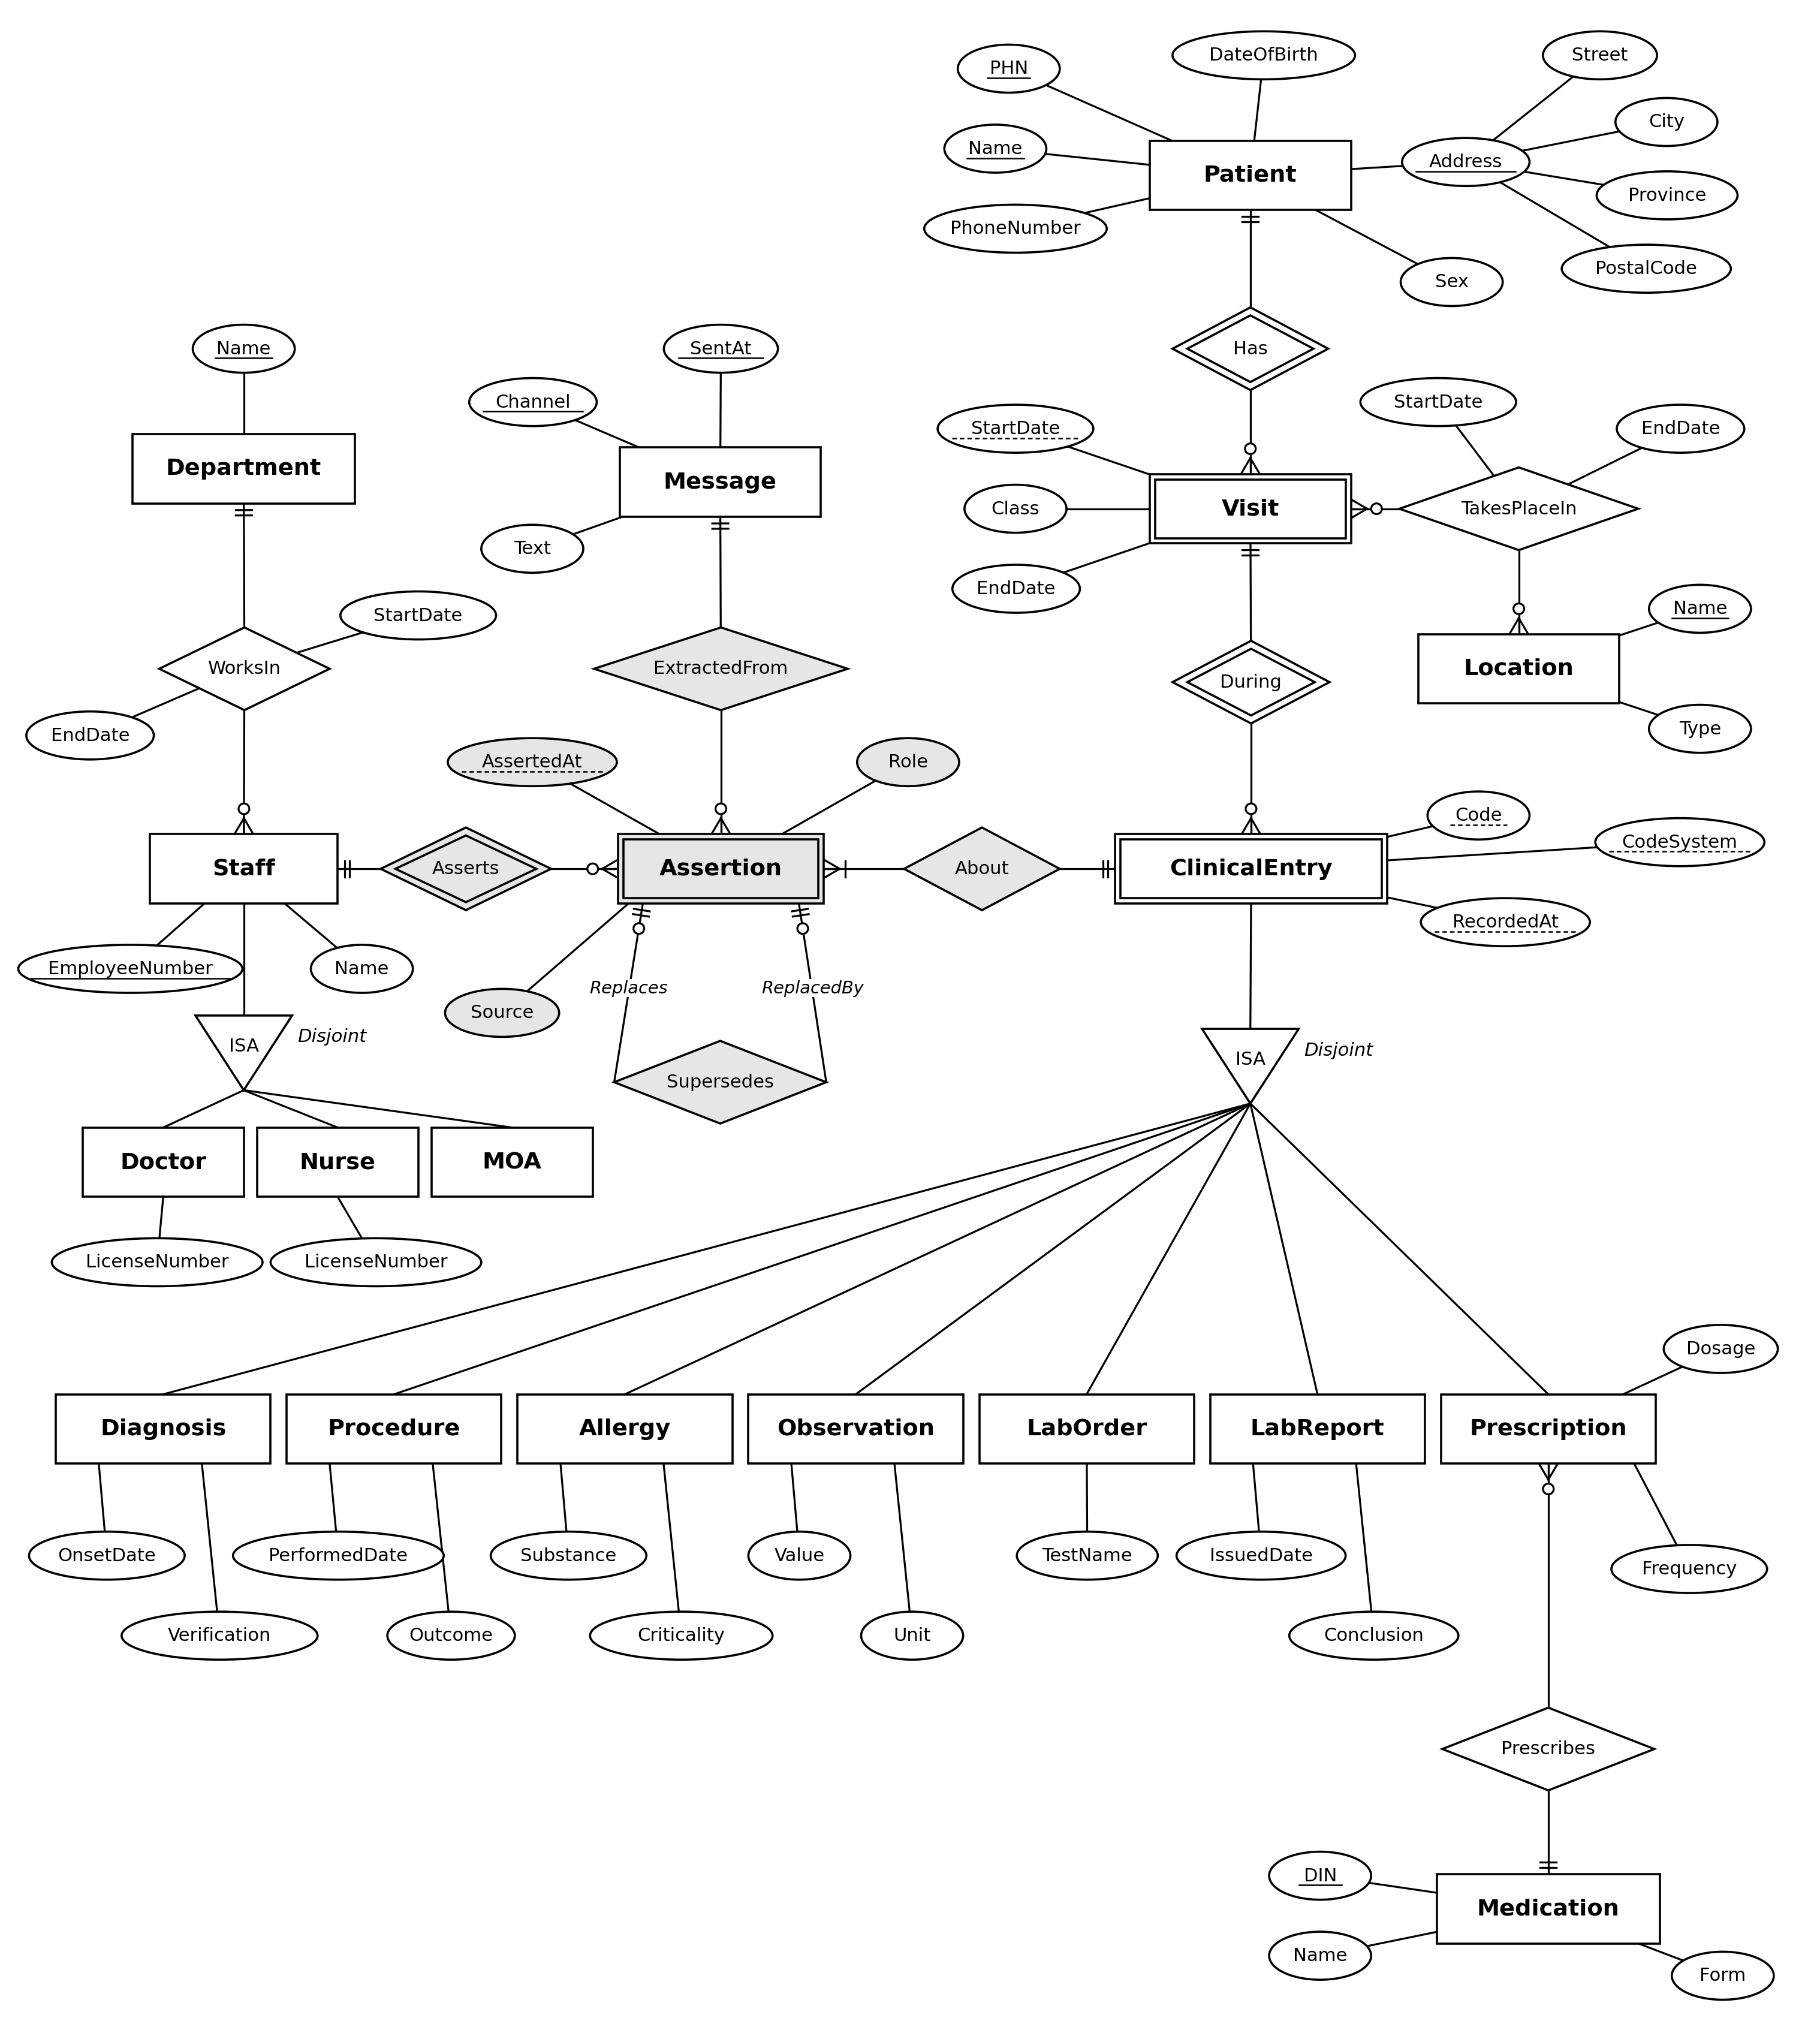
\includegraphics[width=\textwidth,height=0.88\textheight,keepaspectratio]{figures/TRIAD_ERD.png}
\caption{The draft version of our project's ER diagram. The whole model is our design; grey marks where TRIAD's novelty concentrates: who asserted each entry and in what role (Asserts), whether it came from a staff member or an agent acting for them (Source), the entry asserted (About), revision (Supersedes), and the message each assertion was extracted from (ExtractedFrom). White entities take their names from FHIR R4. Double boxes are weak entities; a solid underline marks a key and a dashed underline a partial key. Both IS-A hierarchies are disjoint. The draw.io source is in the repository.}
\label{fig:erd}
\end{figure*}

% ---------------------------------------------------------------
% APPENDIX: original text before AI-assisted editing (Level C).
% Does not count toward the page limit.
% ---------------------------------------------------------------
\clearpage
\onecolumn
\appendix
\section{Original Work Before AI-Assisted Editing}
Per the Level C guideline, this appendix contains the authors' original text
before AI-assisted editing. Sections A.1--A.6 are by Asish A. George. They are
spoken transcripts; AI (Claude) removed filler words, corrected
mis-transcribed words, and joined fragments into complete sentences, without
changing what was said. A.1 also includes his written clarifications. AI was
also used to locate and explain sources and to format the LaTeX.
Sections A.7--A.9 are by Mohamed Khaled. They are spoken transcripts; AI
(Claude) removed filler words and repeated phrases and reordered fragments,
without changing what was said. AI also rendered the ER diagram in draw.io from
his design.
Section A.10 is Mohamed Khaled's spoken draft of the introduction, prepared the same way.
The abstract was assembled by AI from Mohamed Khaled's own wording in the introduction and Section 3, then revised at his direction to add agent authorship and accessibility; it has no separate original.

\subsection{History: Transcript and Clarifications}
This section is about the history of electronic, or medical, records in
general. The earliest case of recording was a papyrus text from 1600 BC
describing a surgery that was done in Egypt. That was one of the earliest
records. Later, there were the Hippocratic school records from the 5th century
BC, and there were health records in between that linked all of this together.
In the late 19th century, Harvard Medical School had medical records
consisting of sections for family history, patient habits, and other data, so
health records became more and more viable. In the process of making records
more active, a clinic number was added, and standardized clinical data was
added. Over the years, the electronic medium was brought into the picture. In
2001, there was the Clinical Document Architecture, a standardized way to use
electronic health data within the system. There were also different exchange
standards in place. However, there was an established study from 2011 on EHRs,
which found that 50 percent of physicians in the United States have an EHR,
but only half of the studies showed a positive impact of having an EHR; some
showed a negative impact, and others found no impact at all. The common
critiques of EHRs are that they are not interoperable and that they are
costly. Those are a few of the cases against EHRs. In 2011, there was a
proposal for FHIR, which is the interoperability standard for health records.
In 2019 the implementation was completed, and by 2020 the US required all EHRs
to provide FHIR APIs for interoperability. But the problem with FHIR is that it
is too lenient. We have to build our own data pipeline, and we have to have
systems that provide FHIR mappings. If we want to build an AI-first approach
that uses these interoperability standards, there are questions about
authorship and the traceability of who updated what, with the history of
changes. That is not there. openEHR is another such standard, in which
different records of data are stored.

\medskip
\noindent\textit{Written clarifications:}
\begin{enumerate}
\item Gillum 2013 describes how Walter Cannon brought the case-history method
from Harvard Law School to Harvard Medical School, and lists the sections of
late-19th-century medical records. 
\item The clinic number was introduced at St Mary's Hospital and the Mayo
Clinic by Henry S. Plummer (1874--1937). Each new patient was assigned a clinic
number.
\item CDA Release 1.0 was published in November 2000 as an ANSI-approved HL7
standard.
\item The study is Lau F, Price M, Boyd J, Partridge C, Bell H, Raworth R,
``Impact of electronic medical record on physician practice in office
settings: a systematic review.''
\item FHIR R4 was released in December 2018.
\item The 2020 requirement should refer to certified health IT, not all EHRs.
\item The papyrus is an Egyptian case report on surgery dating to 1600 BC.
\end{enumerate}

\subsection{Prior Work Opening: Transcript}
For this literature review, we searched different communities and bodies to
find the standards and data models that are available in industry and in the
world. We searched global standards bodies and the academic research side. We
also looked at government organizations and programs, and at the industry best
practices that applications normally use for propagating health records. What
we found was that data models are present at different levels. There is a set
of clinical data models, and there are data models specific to provenance and
change. That was level one, where we have a domain-level decision. Within the
clinical records, we have different data models based on purpose. The first
are operational models, which are used in day-to-day industry activities, and
then there are research and analytical models, used for different research
purposes. For example, the operational models are models like FHIR and
openEHR, whereas the research and analytical models are MIMIC-IV and OMOP CDM,
which are academic models present for different research purposes. We
compared the different models in the study, and we were able to find
differences specific to the use case we are trying to build for. The areas we
found most interesting were authorship (who added what content, and when), the
revision or versioning of the content itself, the time of content addition,
and the enforcement of who is doing what. These were the features most
relevant to us, and that is what we looked at.

\subsection{Operational Models: Transcript}
Within operational models, we are looking at two data models: FHIR and
openEHR. These two are commonly used data models for clinical record exchange
within the industry. FHIR is an interoperability standard, which is
relationship-centric and resource-centric: every entity is resource-based. On
the other side, openEHR is built on versioned compositions, so the composition
is the root, or central, entity in openEHR. Where FHIR deals with
interoperability, openEHR is mainly about long-term, patient-centric records.
The benefit of openEHR is storing the data, whereas FHIR is about the
transferability of data. openEHR actually has integrations with FHIR, so
openEHR can send data through FHIR to surrounding applications. openEHR has a
very good authorship recording mechanism, where every composition needs a
composer, and this is mandatory, whereas in FHIR authorship is a reference to
a resource. Versioning is also a key part of openEHR, because it is long-term
storage. Versioned data is immutable, and there is no overwrite in place, so
openEHR is very strict in that case. It also has a separate time context:
audit time and clinical time are different in openEHR. Similar mechanisms are
also available in FHIR, but there are three levels of time-based mechanisms
there, so that data can be more accessible in different areas. Both FHIR and
openEHR use JSON and XML as their primary data formats, and both are typed:
FHIR has typed resources as such, and openEHR is object-oriented in nature.
Those are the two main operational data models present in the industry.

\subsection{Research and Analytical Models: Transcript}
Research and analytical data models are mainly released for research
purposes. MIMIC-IV is a clinical research dataset, whereas OMOP CDM is more of
a health analytics and observational dataset. In OMOP, the central entity is
the person, and everything flows down from the person entity, whereas in
MIMIC-IV the patient and the encounter are the two main central entities.
These are more for research purposes, so neither of them has a formal
authorship mechanism, because mostly it is generated data or de-identified
records. Even if they have provider IDs or authors, they are not of any value.
There is also no recording time for either, because it is generated data; even
where time is there, it is more for namesake. Both of them are available as
relational databases. MIMIC-IV is distributed as CSV files, which we can
import and use as tables, whereas OMOP has SQL-compatible data types for us to
use directly. That is about the academic data models that were present for us.

\subsection{Time, Provenance, and Change: Transcript}
For our project specifically, the factors that matter quite a lot are the time
of change, the version of content, and the ability to prove who changed what
content and at what time. Across these four models, we were able to observe
different things. First, different models handle provenance in different ways.
For example, openEHR keeps every version of a record as versioned
compositions, so that it can track each element. At the same time, the
negative part is that it is not enforced at the schema level; the application
layer has to enforce it. On the other side, in FHIR, every resource has an
optional layer for who the author can be, but it is never enforced. The
research and analytical models are mainly observational data, so these
factors do not matter as much. In the observational datasets, we can see that
we have more patient-centric entities, whereas in the other standards we do
not have a patient-centric approach. Along with that, these standards are not
fully RDF-compatible. There are small experiments going on with openEHR, where
certain people have tried to make it RDF-compatible, but it is not fully there
yet. With our project, what we would like to do is make TRIAD in such a way
that you can determine the authorship and the time of change definitively,
with authority. It should be a more agent-friendly and RDF-compatible design,
so that the whole thing works together as a single unit.

\subsection{PROV-O and Zep: Transcript}
Other data models and methods that we evaluated in this phase include PROV-O,
which is a standard to represent and interchange provenance information. Here,
the central entities are the entity, activity, and agent triad. It is an
RDF-based, RDF- and OWL-compatible way of representing data. It is not a
clinical data model, but it has a way of versioning data that we would like to
use in our system, and we want to bring something like it in. There is also a
paper called Zep, where the Zep library, which uses Graphiti as its core, shows
how facts are superseded over time: old facts are invalidated rather than
deleted, using timestamps. Zep is not clinical; it is an agent memory layer.
We could use something like Zep's timestamp-based superseding mechanism and
bring it into the clinical space for a faster and more accurate agent
approach.


\subsection{Positioning, the Gap: Transcript}
The gap is that medical data moves between different people: from the patient himself, to the MOA, then to the nurse, and finally it reaches the doctor. This movement of information has two problems. First, this information is mostly natural language, and when it gets assigned to a database, more information can get lost between the transfers. Second, we have inconsistencies over time, especially knowing that the patient can come multiple times and can change his words or add things. We end up with all this information about a patient, and most of it is just updates of the old information, but we don't know that, we just add it, so we have inconsistencies over time. There is also no accountability: if the MOA missed something or the nurse added something, we don't know whether it was the nurse's addition or the MOA's omission. We have no accountability and no traceability.

\subsection{Positioning, What TRIAD Adds: Transcript}
It has two things. First, authorship on each and every fact: this fact was said by the patient himself, this fact was added by the MOA, this fact was added by the nurse, this fact was removed by the doctor. We have authorship on every single fact. For example, the nurse can add things, and we want to know this is the nurse's recommendation; we don't want it mixed with what the patient actually said. Hand in hand with that comes supersession: we have who changed what and who did what. We keep the old version, so when a fact changes, we have the old one and the changed fact. That gives us traceability of what could get lost, and it removes contradictions, because the current fact is a new one we can pull faster, and we still have the backup.

\subsection{Positioning, the Structure: Transcript}
We have a main entity, the Assertion. This Assertion has three binary relationships, with the Message, the Staff, and the ClinicalFact, because we want to know who asserted it (Staff), what specific fact was asserted (ClinicalFact), and from what message. So we have full authorship and full traceability. This entity also has a unary relationship, Supersedes, which records what got replaced by what.

\subsection{Introduction: Transcript}
The problem with clinical data is that it is mostly natural language, and it can also be reported on paper. We then had a whole era of designing databases and data-structuring techniques to shape it in structured ways that make the data line up properly. But there was no intentional focus on traceability, accountability and authorization, especially when their absence can cause very big problems, like inconsistencies. A patient's diagnosis can change in a second. Medications can change, reports can change, a nurse can add recommendations. Things go around from the MOA to the nurse to the doctor, and back. Across this whole pipeline the information keeps going forward and backward, many things get lost, and many things get changed over time, so we have inconsistent or redundant data. From all these inconsistencies we have two problems. First, we can miss things: by the time the information reaches the doctor, it might be incomplete. Second, we might have inconsistencies we cannot resolve, because we do not know which is the newest version or who made an edit. The nurse can add things the MOA did not add, and the nurse might add something wrong, without accountability for who added it or who said it. We have no way of knowing whether this is the patient, an edit, a recommendation, or an actual update. So we have the information, but we do not know how to trace it to somebody, how important it is, or how accurate it is.

\end{document}
